\documentclass{article}
\usepackage[utf8]{inputenc}
\usepackage {mathtools, graphicx, amsfonts, amssymb, comment}
\usepackage{enumerate}
\usepackage{geometry}
\usepackage{subcaption}
\usepackage{float}

\geometry{margin=1.25in}

% http://tex.stackexchange.com/questions/65849/confusion-onehalfspacing-vs-spacing-vs-word-vs-the-world
\linespread{1.25}

\title{Math 414 Final Project}
\author{Matt Gaikema \\ Will Argueta}
\date{April 2016}

\begin{document}

\maketitle

%%%%%%%%%%%%%%%%
% INTRODUCTION %
%%%%%%%%%%%%%%%%
\section{Introduction}
% https://en.wikipedia.org/wiki/Wavelet_transform

In order to efficiently send and receive images, it is often useful to compress them.
One of the many ways of accomplishing this is through wavelets.

There are two types of image compression: lossy and lossless.
\textbf{Lossless} compression means that every bit of information is recovered from the compressed data,
while \textbf{lossy} compression occurs when redundant information is eliminated.
The GIF is an example of lossless compression, while the JPEG is lossy.

Wavelets are also useful for detecting and removing noise from an image.
\ref{fig:noisy} gives an example of a noisy image.
\begin{figure}
    \centering
    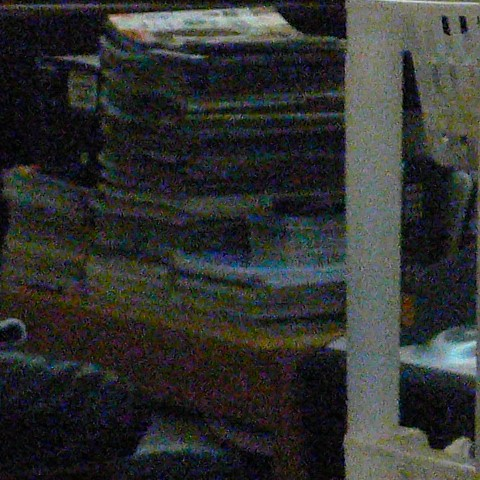
\includegraphics[scale=0.4]{Highimgnoise.jpg}
    \caption{An image with a lot of noise}
    \label{fig:noisy}
\end{figure}


%%%%%%%%%%%%%%%%%%%%%%%%%%%
% MATHEMATICAL BACKGROUND %
%%%%%%%%%%%%%%%%%%%%%%%%%%%
\section{Mathematical Background}
% https://en.wikipedia.org/wiki/JPEG_2000
% http://cs.haifa.ac.il/hagit/courses/seminars/wavelets/Presentations/Lecture09_Denoising.pdf

The wavelet transform on an image produces as many coefficients as there are pixels.


%%%%%%%%%%%%%%%
% APPLICATION %
%%%%%%%%%%%%%%%
\section{Application}


%%%%%%%%%%%%%%
% CONCLUSION %
%%%%%%%%%%%%%%
\section{Conclusion}


%%%%%%%%%%%%%%
% REFERENCES %
%%%%%%%%%%%%%%
\section{References}

\end{document}
